\documentclass[12pt]{report}
\usepackage{fontspec}
\usepackage{fullpage}
\usepackage{hyperref}
\usepackage{array}
\usepackage{url}
\usepackage{amsmath}
\usepackage{pgfplotstable}
\usepackage{algorithm2e}
\usepackage{multirow}
\usepackage{subcaption}
\usepackage{color}
\usepackage{adjustbox}
\usepackage{tikz}
\usepackage{tikz-dependency}
\usepackage{titling}
\usepackage{pdfpages}
\usetikzlibrary{shapes,fit,calc,er,positioning,intersections,decorations.shapes,mindmap,trees}
\tikzset{decorate sep/.style 2 args={decorate,decoration={shape backgrounds,shape=circle,
      shape size=#1,shape sep=#2}}}

\newfontfamily\hebfont[Script=Hebrew, Scale=MatchUppercase]{FreeSans}
\newcommand{\heb}[1]{\bgroup\textdir TRT\hebfont #1\egroup}

\title{
\textbf{Universal Semantic Parsing with Neural Networks} \\
\vspace{2cm}
{\large Thesis submitted for the degree of \\
``Doctor of Philosophy''}
}
\author{
By \\
Daniel Hershcovich
\vspace{2cm}
}
\date{
Submitted to the Senate of the Hebrew University \\
February, 2019
}

\begin{document}

\maketitle
\clearpage
\title{}
\author{
This work was carried out under the supervision of: \\
Prof. Ari Rappoport and Dr. Omri Abend
}
\date{}
\maketitle


\section{Introduction}\label{sec:introduction}

Semantic applications in natural language processing (e.g., machine translation)
require understanding the meaning of text.
Syntactic representations suffer from limitations, since they do not
represent semantic structure directly,
which semantic annotation schemes attempt to do.
In order to represent the full range of semantic structures exhibited by
natural language, three properties should be supported: reentrancy,
representing arguments shared between predicates (Figure~\ref{fig:graduation});
non-terminal nodes for multi-word units (Figure~\ref{fig:home});
and discontinuity of semantic units in the text (Figure~\ref{fig:gave}).
The only semantic annotation scheme that supports the combination of these criteria is UCCA
\cite{abend2013universal}.

\begin{figure}[ht]\small
  \begin{subfigure}{.6\textwidth}
  \parbox{.1\textwidth}{\caption{}\label{fig:graduation}}
  \parbox{.3\textwidth}{
  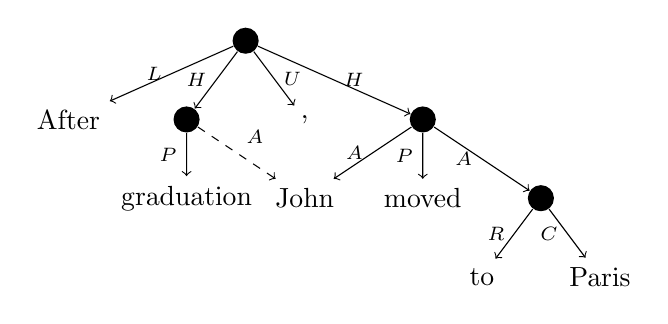
\begin{tikzpicture}[level distance=10mm, ->]
    \node (ROOT) [fill=black, circle] {}
      child {node (After) {After} edge from parent node[left] {\scriptsize $L$}}
      child {node (graduation) [fill=black, circle] {}
      {
        child {node {graduation} edge from parent node[left] {\scriptsize $P$}}
      } edge from parent node[left] {\scriptsize $H$} }
      child {node {,} edge from parent node[right] {\scriptsize $U$}}
      child {node (moved) [fill=black, circle] {}
      {
        child {node (John) {John} edge from parent node[left] {\scriptsize $A$}}
        child {node {moved} edge from parent node[left] {\scriptsize $P$}}
        child {node [fill=black, circle] {}
        {
          child {node {to} edge from parent node[left] {\scriptsize $R$}}
          child {node {Paris} edge from parent node[left] {\scriptsize $C$}}
        } edge from parent node[left] {\scriptsize $A$} }
      } edge from parent node[right] {\scriptsize $H$} }
      ;
    \draw[dashed,->] (graduation) to node [auto] {\scriptsize $A$} (John);
  \end{tikzpicture}
  }
  \end{subfigure}
  \begin{subfigure}{.4\textwidth}
  \parbox{.1\textwidth}{\caption{}\label{fig:home}}
  \parbox{.3\textwidth}{
  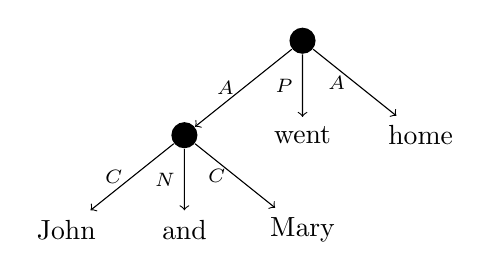
\begin{tikzpicture}[level distance=12mm, ->,
      every node/.append style={midway}]
    \node (ROOT) [fill=black, circle] {}
      child {node [fill=black, circle] {}
      {
        child {node {John} edge from parent node[left] {\scriptsize $C$}}
        child {node {and} edge from parent node[left] {\scriptsize $N$}}
        child {node {Mary} edge from parent node[left] {\scriptsize $C$}}
      } edge from parent node[left] {\scriptsize $A$} }
      child {node {went} edge from parent node[left] {\scriptsize $P$}}
      child {node {home} edge from parent node[left] {\scriptsize $A$}}
      ;
  \end{tikzpicture}
  }
  \end{subfigure}
  \begin{subfigure}{.4\textwidth}
  \parbox{.1\textwidth}{\caption{}\label{fig:gave}}
  \parbox{.3\textwidth}{
  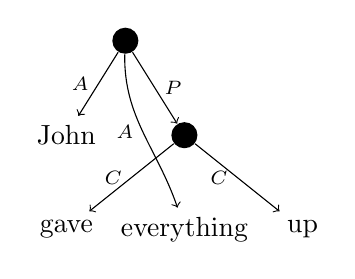
\begin{tikzpicture}[level distance=12mm, ->,
      every node/.append style={midway}]
    \node (ROOT) [fill=black, circle] {}
      child {node {John} edge from parent node[left] {\scriptsize $A$}}
      child {node [fill=black, circle] {}
      {
      	child {node {gave} edge from parent node[left] {\scriptsize $C$}}
      	child {node (everything) {everything} edge from parent[white]}
      	child {node {up} edge from parent node[left] {\scriptsize $C$}}
      } edge from parent node[right] {\scriptsize $P$} }
      ;
    \draw[bend right,->] (ROOT) to[out=-20, in=180] node [left] {\scriptsize $A$} (everything);
  \end{tikzpicture}
  }
  \end{subfigure}
  \begin{subfigure}{.6\textwidth}
  \parbox{.1\textwidth}{\caption{}\label{fig:shower}}
  \parbox{.3\textwidth}{
  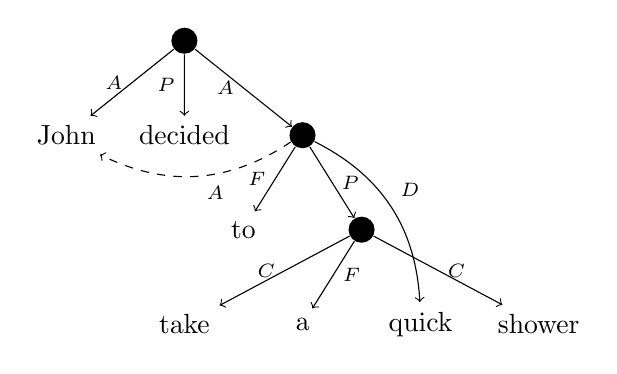
\begin{tikzpicture}[level distance=12mm, ->,
      every node/.append style={midway}]
    \node (ROOT) [fill=black, circle] {}
      child {node (John) {John} edge from parent node[left] {\scriptsize $A$}}
      child {node {decided} edge from parent node[left] {\scriptsize $P$}}
      child {node (totakeaquickshower) [fill=black, circle] {}
      {
        child {node {to} edge from parent node[left] {\scriptsize $F$}}
        child {node [fill=black, circle] {}
        {
          child {node {take} edge from parent node[left] {\scriptsize $C$}}
          child {node {a} edge from parent node[right] {\scriptsize $F$}}
          child {node (quick) {quick} edge from parent[white]}
          child {node {shower} edge from parent node[right] {\scriptsize $C$}}
        } edge from parent node[right] {\scriptsize $P$} }
      } edge from parent node[left] {\scriptsize $A$} }
      ;
    \draw[bend left,dashed,->] (totakeaquickshower) to node [auto] {\scriptsize $A$} (John);
    \draw[bend left,->] (totakeaquickshower) to node [auto] {\scriptsize $D$} (quick);
  \end{tikzpicture}
  }
  \end{subfigure}
  \caption{\label{fig:examples}
    UCCA examples.
    (\subref{fig:graduation}) includes a remote edge (dashed),
    resulting in ``John'' having two parents.
    (\subref{fig:home}) includes a coordination construction (``John and Mary'').
    (\subref{fig:gave}) includes a discontinuous unit (``gave ... up'').
    (\subref{fig:shower}) includes both a remote edge and a discontinuous unit (``take a ... shower'').
    Legend: $P$ -- Process (a Scene's main relation), $A$ -- Participant,
    $L$ -- inter-scene Linker, $H$ -- Parallel Scene, $C$ -- Center, $D$ -- Adverbial,
    $R$ -- Relator, $N$ -- Connector, $U$ -- Punctuation, $F$ -- Function unit.
  }
\end{figure}

Universal Cognitive Conceptual Annotation (UCCA)
is a cross-linguistically applicable semantic representation scheme.
It covers the predicate-argument
structures evoked by predicates of all grammatical categories, the inter-relations between them,
as well as other major linguistic phenomena.
UCCA has demonstrated applicability to multiple languages,
rapid annotation \cite{abend2017uccaapp},
stability in translation \cite{sulem2015conceptual}
and benefit for various applications
\cite{birch2016hume,choshen2018usim,sulem2018samsa,sulem2018simple}.

While semantic representation schemes are different in form and focus,
much of their semantic content is shared \cite{abend2017state}.
Recent work in semantic parsing has targeted
Abstract Meaning Representation \cite{banarescu2013abstract} and
Semantic Dependencies \cite{oepen2016towards}.
Universal Dependencies \cite{nivre2016universal}
is a \textit{syntactic} dependency scheme aiming for cross-lingual consistency,
whose annotation is often similar to the common practice in semantic treebanks
(Figure~\ref{fig:original_example_ud}).

\begin{figure}[th]
  \centering
    \begin{dependency}[text only label, label style={above,font=\tt}, font=\small]
    \begin{deptext}[column sep=.8em,ampersand replacement=\^]
    After \^ graduation \^ , \^ John \^ moved \^ to \^ Paris \\
    \end{deptext}
        \depedge[edge unit distance=1ex]{2}{1}{case}
        \depedge[edge unit distance=1ex]{2}{3}{punct}
        \depedge[edge unit distance=1ex]{5}{4}{nsubj}
        \depedge[edge unit distance=1ex, edge end x offset=-2pt]{5}{2}{obl}
        \depedge[edge unit distance=1ex]{7}{6}{case}
        \deproot[edge unit distance=1.5ex]{5}{root}
        \depedge[edge unit distance=1.5ex]{5}{7}{obl}
    \end{dependency}
\caption{Example UD tree, demonstrating practices common in semantic annotation:
linking content words to content words, and the preference of lexical heads over functional ones.
\label{fig:original_example_ud}}
\end{figure}

My research is concerned with learning to parse UCCA graphs from text, representing its semantics.
I introduce a general graph parser,
and investigate the relationship with other representations to find beneficial commonalities and
differences highlighting the potential utility of semantic parsers for text understanding applications.
The analysis also exposes challenges semantic parsers must address,
and potential sources for improvement.

\section{Goals}\label{sec:goals}

In my research, I pursue the following goals:

\begin{itemize}
  \item Developing techniques for general graph parsing.
    Specifically, devising a method for automatic prediction of UCCA
    structure given plain text.
  \item Investigating and quantifying the relationship between the content
    captured in UCCA and other semantic or syntactic representations.
  \item Taking advantage of the similarities to other schemes,
    to improve UCCA parsing by learning common distinctions.
\end{itemize}


\section{Methods}\label{sec:methods}

\subsection{Transition-Based Parsing}\label{sec:transition_based}

Transition-based parsers \cite{Nivre03anefficient} build trees or graphs
as they scan the text incrementally.
The parse is created by applying a \textit{transition} at each step to the parser state,
defined using a buffer of tokens and nodes to be processed,
a stack of nodes currently being processed,
and a graph of constructed nodes and labeled edges.
A classifier is used at each step to select the next transition based on features
that encode the parser's current state.
During training, an oracle creates training instances for the classifier,
based on the gold-standard annotation.

The transition-based approach has produced some of the best
results in syntactic dependency parsing
\cite{kiperwasser2016simple,andor2016globally}, and has also demonstrated
strong performance in a variety of other semantic and syntactic settings
\cite{maier2015discontinuous,damonte-17}.
Transition-based methods are a natural starting point for UCCA parsing,
as the set of distinctions it represents is similar in spirit to the distinctions
conveyed by dependency schemes.


\subsection{Neural Networks}\label{sec:neural_networks}

Neural networks are powerful machine learning models.
They have yielded state-of-the-art results in many fields,
including natural language processing \cite{goldberg2016primer}.
Inspired by the brain's computation mechanism,
artificial neural networks operate on dense input representations
by a combination of linear and non-linear transformations.

Language data is commonly manifested as sequences
(e.g., sentences are sequences of words).
Recurrent neural networks \cite{elman1990finding} allow representing
arbitrarily sized sequences in a fixed-size vector,
without ignoring the structured properties of the input.
A specific flavor called Long Short Term Memory
(LSTM) is very common as it learns relatively long-term dependencies.
A bidirectional recurrent neural network, such as a BiLSTM,
takes into account both the past and future.


\subsection{Multitask Learning}\label{sec:multitask}

Multitask learning \cite{caruana1998multitask} allows exploiting the overlap between tasks
to effectively extend the training data, 
and has greatly advanced with neural networks and representation learning.
It has been used over the years for NLP tasks with varying degrees of similarity.

Neural multitask learning has mostly been effective in tackling formally similar
tasks \cite{P16-2038},
including
multilingual syntactic dependency parsing \cite{Q16-1031,guo2016exploiting},
as well as multilingual \cite{duong2017multilingual},
and cross-domain semantic parsing \cite{herzig-berant:2017:Short,W17-2607}.

Sharing parameters with a low-level task
has shown great benefit for transition-based syntactic parsing
\cite{bohnet2012transition,Zhang2016StackpropagationIR,constant-nivre:2016:P16-1,more2016joint}.
Recent work has achieved state-of-the-art results in multiple NLP tasks
by jointly learning the tasks forming the NLP standard pipeline using 
a single neural model \cite{collobert2011natural,D17-1206},
thereby avoiding cascading errors, common in pipelines.


\section{Experiments}\label{sec:experiments}

\paragraph{Data.}

Experiments are performed on the English Wikipedia UCCA corpus (Wiki),
the \textit{Twenty Thousand Leagues Under the Sea} UCCA corpora (20K),
annotated in English, French and German;
LDC2017T10 for AMR;
the DM representation from SDP 2016;
and all English, French and German treebanks from UD v2.1.


\paragraph{Evaluation.}
Comparing UCCA structures
$G_p=(V_p,E_p,\ell_p)$ and $G_g=(V_g,E_g,\ell_g)$,
over the same sequence of terminals $W = \{w_1,\ldots,w_n\}$
is done as follows.
For an edge $e=(u,v)$ in either graph, its yield $y(e) \subseteq W$ is the
set of terminals in $W$ that are descendants of $v$.
Define the set of \textit{mutual edges} between $G_p$ and $G_g$:
\[
    M(G_p,G_g) =
    \left\{(e_1,e_2) \in E_p \times E_g \;|\;
    y(e_1) = y(e_2) \wedge \ell_p(e_1)=\ell_g(e_2)\right\}
\]

Labeled precision and recall are defined by dividing $|M(G_p,G_g)|$ by $|E_p|$ and $|E_g|$, respectively,
and F-score by taking their harmonic mean.
Two variants are reported: one where we consider only primary edges,
and another for remote edges


\paragraph{Settings.}

The following settings are explored:
(1) in-domain setting in English, training and testing on Wiki;
(2) out-of-domain setting in English, training on Wiki and testing on 20K;
(3) French in-domain setting, where available training dataset is small,
training and testing on 20K;
(4) German in-domain setting on 20K, with somewhat noisy annotation.
For multitask experiments, we use unlabeled AMR, DM and UD parsing as auxiliary tasks in English,
and unlabeled UD parsing in French and German.

\paragraph{Baselines.}
As no direct comparison with existing parsers is possible,
baselines are bi-lexical dependency graph parsers,
which support reentrancy and discontinuity but not non-terminal nodes;
and \textit{tree approximation}, converting UCCA to (bi-lexical) trees
and evaluating constituency and dependency tree parsers on them.
Baselines are DAGParser \cite{ribeyre-villemontedelaclergerie-seddah:2014:SemEval} and
TurboParser \cite{almeida-martins:2015:SemEval},
two bi-lexical dependency graph parsers;
\textsc{uparse} \cite{maier-lichte:2016:DiscoNLP},
a transition-based constituency parser supporting discontinuous constituents;
and two bi-lexical tree parsers:
MaltParser \cite{nivre2007maltparser},
and the stack LSTM parser \cite{dyer2015transition}.


\paragraph{Results.}

\begin{table}[t]
\centering
\footnotesize
\setlength\tabcolsep{3pt}
\begin{subfigure}{.475\textwidth}
\begin{tabular}{l|lll|lll}
& \multicolumn{3}{c|}{\bf Primary} & \multicolumn{3}{c}{\bf Remote} \\
& \textbf{LP} & \textbf{LR} & \textbf{LF}
& \textbf{LP} & \textbf{LR} & \textbf{LF} \\
\hline
\multicolumn{4}{l|}{\bf English (in-domain)} \\
\multicolumn{4}{l|}{\rule{0pt}{2ex}
Bi-lexical Approximation} \\
DAGParser
& 61.8 & 55.8 & 58.6 & 9.5 & 0.5 & 1 \\
TurboParser
& 57.7 & 46 & 51.2 & 77.8 & 1.8 & 3.7 \\
\hline
\multicolumn{4}{l|}{\rule{0pt}{2ex}
Tree Approximation} \\
\textsc{uparse}
& 60.9 & 61.2 & 61.1 & -- & -- & -- \\
\hline
\multicolumn{4}{l|}{\rule{0pt}{2ex}
Bi-lexical Tree Approximation} \\
MaltParser
& 62.8 & 57.7 & 60.2 & -- & -- & -- \\
LSTM Parser
& 73.2 & 66.9 & 69.9 & -- & -- & -- \\
\hline
Single
& 74.4 & 72.9 & 73.6 & 53 & 50 & 51.5 \\
Multitask &&& \\
AMR
& 74.7 & 72.8 & 73.7 & 48.7 & 51.1 & 49.9 \\
DM
& 75.7 & 73.9 & 74.8 & 54.9 & 53 & \textbf{53.9} \\
UD
& 75 & 73.2 & 74.1 & 49 & 52.7 & 50.8 \\
AMR + DM
& 75.6 & 73.9 & 74.7 & 49.9 & 53 & 51.4 \\
AMR + UD
& 74.9 & 72.7 & 73.8 & 47.1 & 50 & 48.5 \\
DM + UD
& 75.9 & 73.9 & \textbf{74.9} & 48 & 54.8 & 51.2 \\
All
& 75.6 & 73.1 & 74.4 & 50.9 & 53.2 & 52
\end{tabular}\label{tab:id_results}
\vspace{24.5mm}
\end{subfigure}
\hfill
\begin{subfigure}[t]{.475\textwidth}
\begin{tabular}{l|lll|lll}
& \multicolumn{3}{c|}{\bf Primary} & \multicolumn{3}{c}{\bf Remote} \\
& \textbf{LP} & \textbf{LR} & \textbf{LF}
& \textbf{LP} & \textbf{LR} & \textbf{LF} \\
\hline
\multicolumn{4}{l|}{\bf English (out-of-domain)} \\
\multicolumn{4}{l|}{\rule{0pt}{2ex}
Bi-lexical Approximation} \\
DAGParser
& 56.4 & 50.6 & 53.4 & -- & 0 & 0 \\
TurboParser
& 50.3 & 37.7 & 43.1 & 100 & 0.4 & 0.8 \\
\hline
\multicolumn{4}{l|}{\rule{0pt}{2ex}
Tree Approximation} \\
\textsc{uparse}
& 52.7 & 52.8 & 52.8 & -- & -- & -- \\
\hline
\multicolumn{4}{l|}{\rule{0pt}{2ex}
Bi-lexical Tree Approximation} \\
MaltParser
& 57.8 & 53 & 55.3 & -- & -- & -- \\
LSTM Parser
& 66.1 & 61.1 & 63.5 & -- & -- & -- \\
\hline
Single
& 69 & 69 & 69 & 41.2 & 19.8 & 26.7 \\
Multitask &&& \\
AMR
& 69.5 & 69.5 & 69.5 & 42.9 & 20.2 & 27.5 \\
DM
& 70.7 & 70.7 & 70.7 & 42.7 & 18.6 & 25.9 \\
UD
& 69.6 & 69.8 & 69.7 & 41.4 & 22 & 28.7 \\
AMR + DM
& 70.7 & 70.2 & 70.5 & 45.8 & 19.4 & 27.3 \\
AMR + UD
& 70.2 & 69.9 & 70 & 45.1 & 21.8 & 29.4 \\
DM + UD
& 70.8 & 70.3 & 70.6 & 41.6 & 21.6 & 28.4 \\
All
& 71.2 & 70.9 & \textbf{71} & 45.1 & 22 & \textbf{29.6} \\
\hline
\multicolumn{4}{l|}{\bf French (in-domain)} & \\
Single & 68.2 & 67 & 67.6 & 26 & \enskip 9.4 & 13.9 \\
UD & 70.3 & 70 & \textbf{70.1} & 43.8 & 13.2 & 20.3 \\
\hline
\multicolumn{4}{l|}{\bf German (in-domain)} & \\
Single & 73.3 & 71.7 & 72.5 & 57.1 & 17.7 & 27.1 \\
UD & 73.7 & 72.6 & \textbf{73.2} & 61.8 & 24.9 & \textbf{35.5}
\end{tabular}\label{tab:ood_results}
\end{subfigure}
\caption{
Labeled precision, recall and F-score (in~\%)
on Wiki (left) and 20K (right).
}\label{tab:results}
\end{table}

Table~\ref{tab:results} presents the results.
The stack LSTM parser obtains the highest primary F-score
among the baseline parsers, with a considerable margin. However,
tree approximation parsers are unable to recover any remote edges,
removed in the conversion.
The bi-lexical DAG parsers are quite limited in this respect as well.
The direct UCCA parser, based on BiLSTMs, outperforms all baselines.
Multitask further improves the primary F-score over the single task parser,
but using all auxiliary tasks contributes less than just DM and UD.
For 20K, improvements from using multitask are even more marked. 
Moreover, the improvement is largely additive.
The best multitask models are significantly better than single-task models,
demonstrating that even a small training set for the main task may suffice,
given enough auxiliary training data (as in French).

\paragraph{Discussion.}

Task similarity is an important factor in multitask learning
\cite{E17-2026,E17-1005}.
Empirical comparison with UD reveals that most content differences between it and UCCA are due to:
  \begin{enumerate}
      \item UCCA's distinction of Scene-evoking words and phrases, absent in UD.
      \item UCCA's distinction between primary relations, secondary relations
        and Participants, in contrast to UD's core/non-core distinction.
      \item Different treatment of multi-word expressions (MWEs),
        where UCCA has a stronger tendency to explicitly mark them.
      \item UCCA's conflation of several syntactic realizations of inter-clause linkage,
        and disambiguation of other cases that UD treats similarly.
   \end{enumerate}

  The differences between the schemes are substantial, and suggest that
  UCCA parsing in particular and semantic parsing in general are likely to benefit
  downstream text understanding applications.
  For example, only 73\% of arguments are shared between UCCA and UD,
  i.e., many semantic participants cannot be recovered from UD.


\section{Challenges}\label{sec:challenges}

\paragraph{Dataset size.}
Models with a large number of parameters typically require very large
training sets.
Since the UCCA datasets are small in relation to other schemes,
training neural network models on them posed a challenge.
While the data is slowly growing and extended to more languages by further labeling efforts,
multitask learning proved to be an effective method to overcome the data scarcity issue.

\paragraph{Scheme comparison.}
While many distinctions are shared between UCCA and other semantic and syntactic schemes,
they are largely obscured by differences in representation format and convention.
Conversion to a common graph format and assimilation of superficial structures
allowed deep inspection of content divergences and convergences.


\section{Future Work}\label{sec:future_work}

The research effort to be included in the PhD thesis was completed on December 10, 2018.

UCCA's merits in providing a cross-linguistically applicable,
broad-coverage annotation will support ongoing efforts to incorporate deeper
semantic structures into a variety of applications, such as machine translation
\cite{jones2012semantics} and summarization \cite{liu2015toward}.
The advantage of UCCA as compared to syntactic annotation schemes for machine translation is apparent,
as translation tends to preserve semantic structure more than syntactic structure \cite{sulem2015conceptual}.
Using UCCA as an intermediate representation is thus likely to achieve outputs that are more
semantically similar to the source.

\chapter{A Transition-Based Directed Acyclic Graph Parser for UCCA}

\includepdf[pages=-]{P17-1104.pdf}

\chapter{Multitask Parsing Across Semantic Representations}

\includepdf[pages=-]{P18-1035.pdf}

\chapter{Universal Dependency Parsing with a General Transition-Based DAG Parser}

\includepdf[pages=-]{K18-2010.pdf}

\chapter{Content Differences in Syntactic and Semantic Representations}

\includepdf[pages=-]{divergences.pdf}


\bibliography{references}
\bibliographystyle{plain}
\end{document}
